\section{Solução desenvolvida}
\label{sec:iotGateway}

Além deste artigo, foi desenvolvida uma solução de software de Smart Gateway IoT que está disponibilizada no Github \cite{IoTGatewayGithub}. Esta seção propõe-se a detalhar os objetivos e decisões arquiteturais. Sendo assim, desenvolveu-se uma solução de Smart Gateway IoT, capaz de receber dados através de uma rede utilizando o protocolo MQTT de um dispositivo previamente cadastro e armazenar essas informações. Os dados recebidos são analisados para um embasamento onde irá definir a execução ou não de um fluxo de notificação através de SMS para um número definido.

\subsection{Tecnologias Utilizadas} 
\begin{itemize}
	\item Node.js v6.x \cite{NodeJS};
	\item TypeScript 2.3 com transpile para ES6 \cite{Typescript};
	\item TSLint 4.x com recomendações gerais padrão \cite{TSLint};
	\item Jest para teste unitário e cobertura \cite{Jest};
	\item Angular 1.6 para o front end da aplicação \cite{AngularJS};
	\item MongoDB \cite{MongoDB}.
	\item MQTT \cite{Mqtt}
	\item Express como framework web Node.js \cite{ExpressJS}
\end{itemize}

O Node.js \cite{NodeJS} foi escolhido por conta de seu baixo consumo de memória e processamento, além da sua característica de Non-Blocking IO \cite{NodeJSNonBlockingIO}, garantindo que possamos servir mais clientes com menos recursos, objetivo essencial para aplicações que podem ser executadas em um Raspberry Pi por exemplo.

A escolha pelo TypeScript \cite{Typescript}, linguagem que é um superset do Javascript padrão foi motivada por garantir uma estrutura tipada, de forma que a manutenção do código fosse facilitada e as regras de negócio pudessem estar ligadas a um contrato de objeto.

Já o AngularJS \cite{AngularJS} foi escolhido, por ser uma tecnologia que funciona com javascript nativo, sem necessidade de nenhum pós-processador para servir a aplicação aos clientes, permitindo o seu uso diretamente entre os arquivos estáticos do mesmo servidor Node.js que expõe a aplicação. Além disso, contou como um ponto para a escolha, a experiência prévia da equipe no desenvolvimento com esta tecnologia.

O MQTT \cite{Mqtt}, abreviação de MQ Telemetry Transport, é um protocolo de comunicação altamente voltado para IoT. Ele foi arquitetado para ser um sistema de mensageria leve do tipo publisher/subscriber, para rodar em dispositivos limitados, tanto do ponto de vista da quantidade de memória para execução do programa, quanto do ponto de vista da conectividade. Redes lentas ou com alta latência não são problemas para esse protocolo. Geralmente, sensores IoT podem residir em locais extremamente hostis do ponto de vista de infra-estrutura de conexão de dados.

\subsection{Modelo de Dados}
O modelo de dados foi concebido com a intenção de tornar as etapas do processo altamente plugáveis e customizáveis no curto e longo prazo, garantindo as funcionalidades básicas do MVP executado e a possibilidade de extensibilidade no futuro com retrocompatibilidade, ver Figura~\ref{fig:modeloDeDados}.

\begin{figure}[h!]
	\begin{center}
		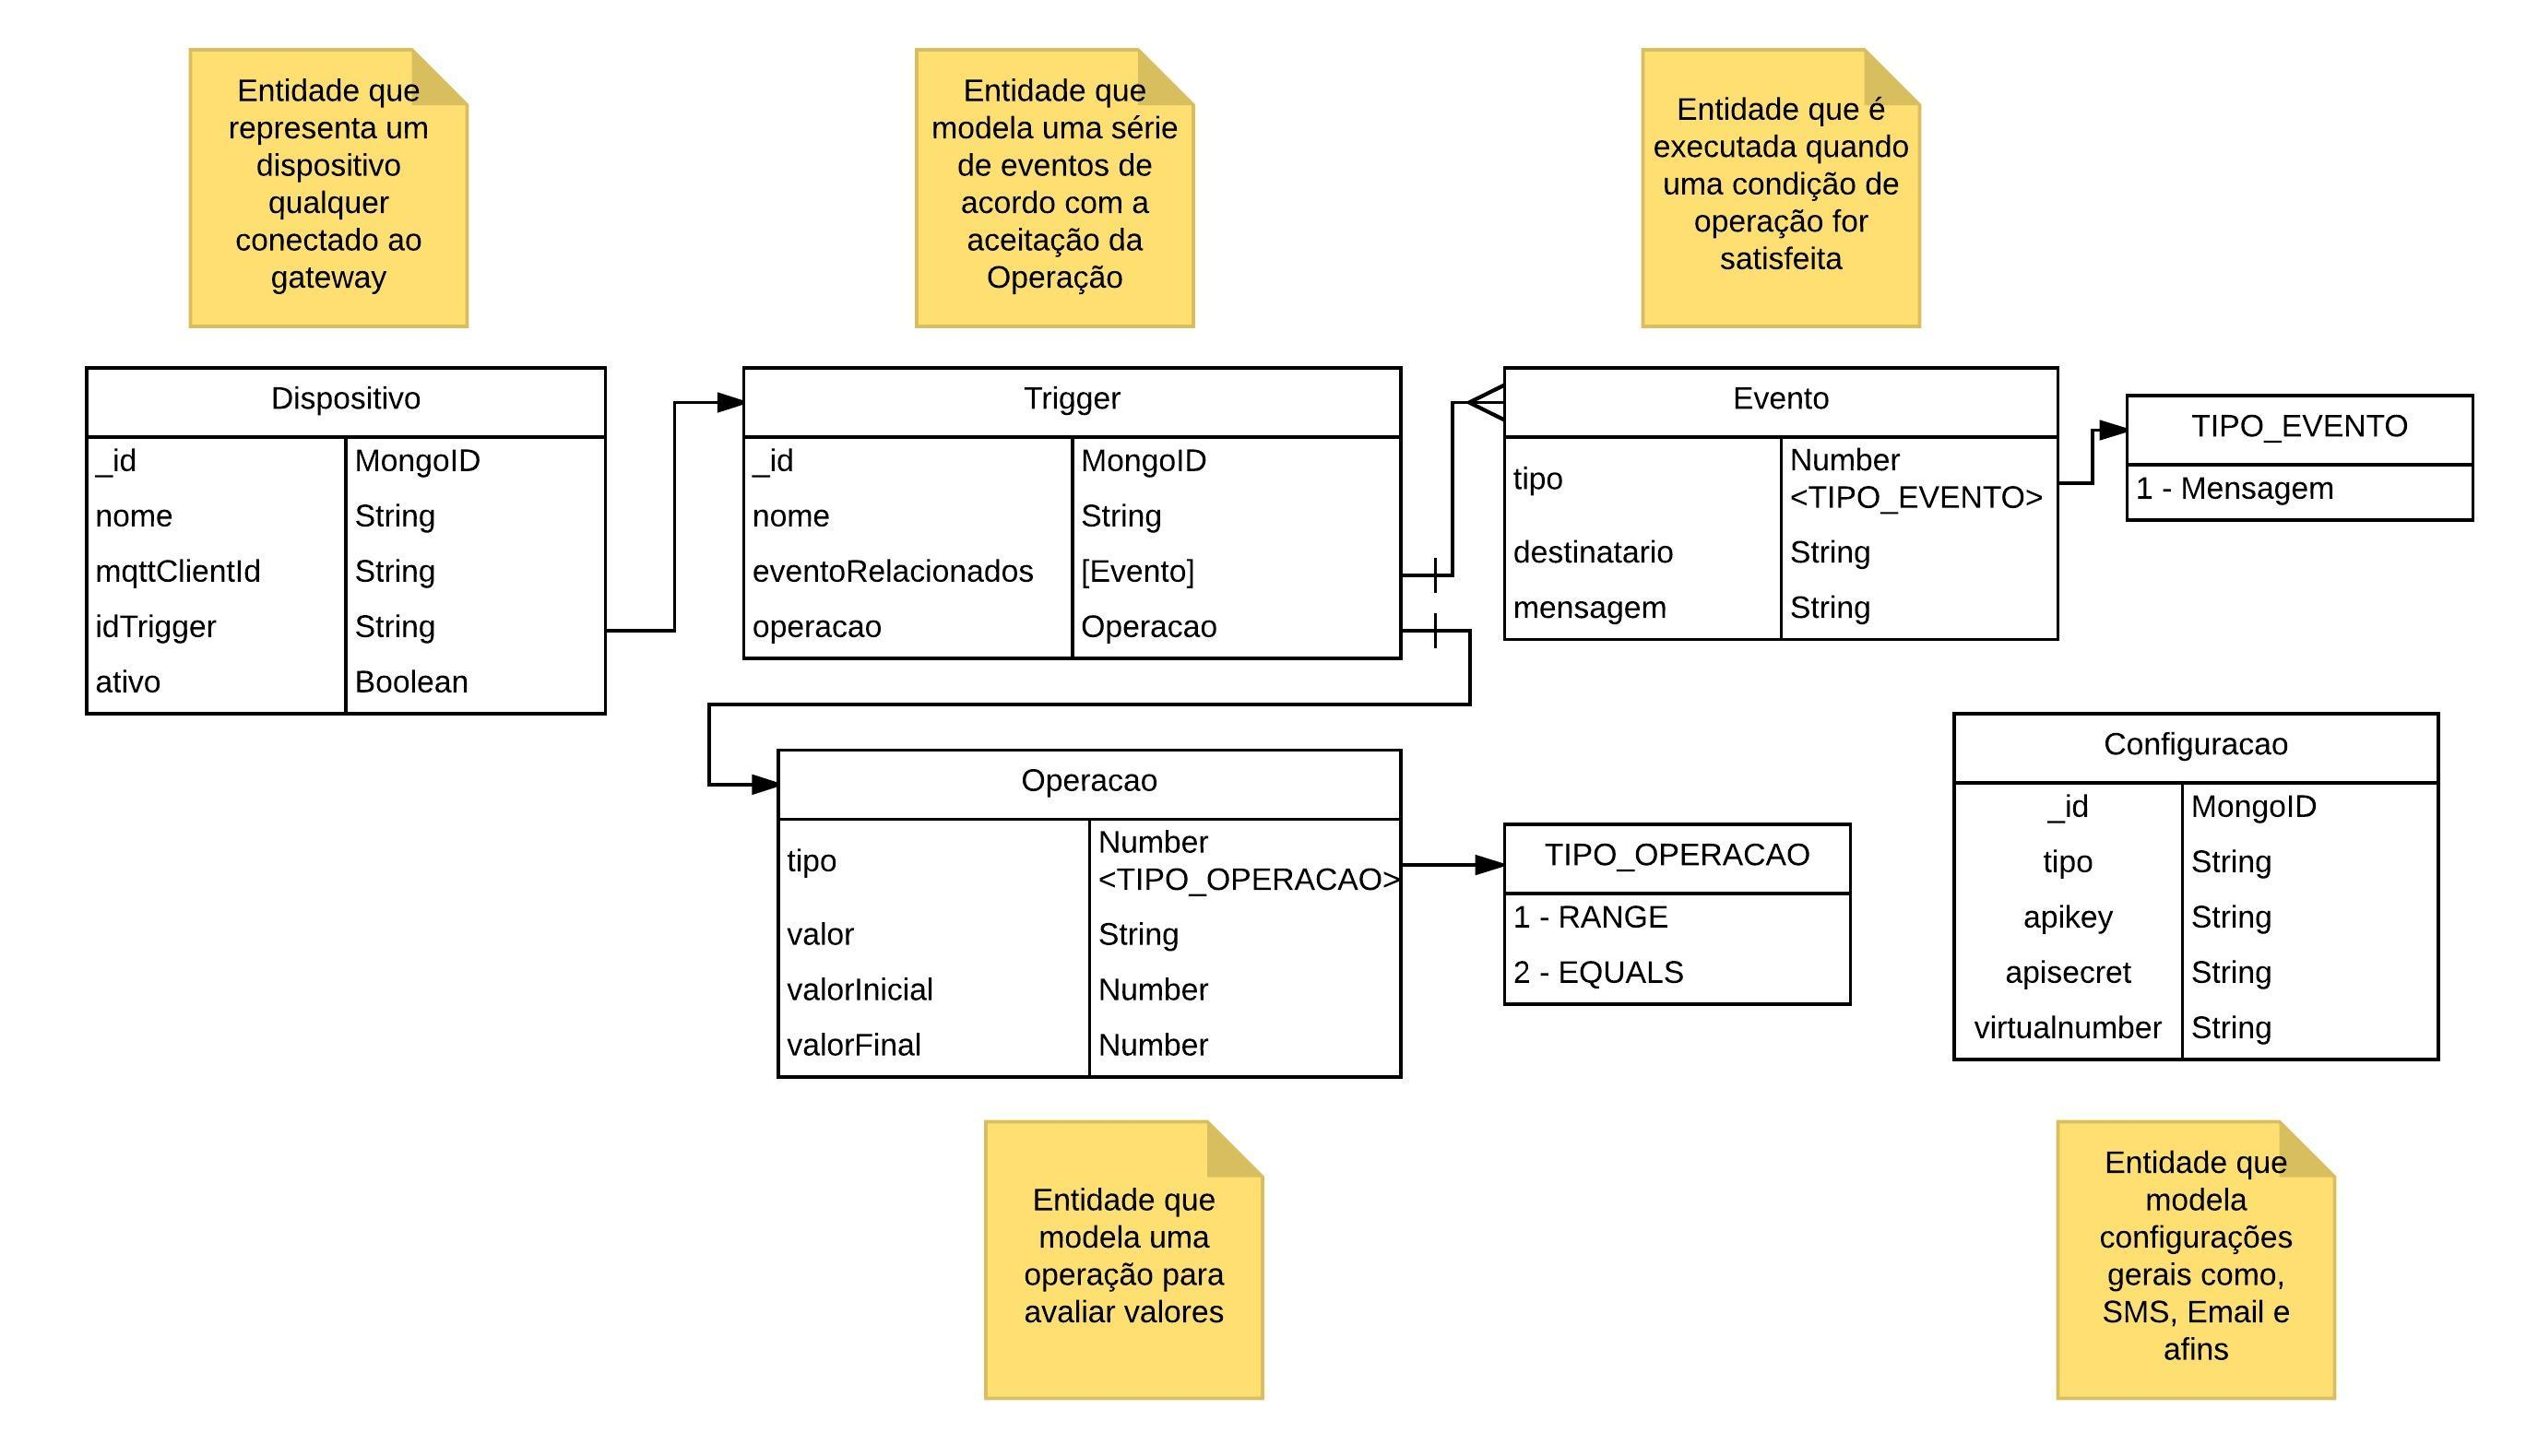
\includegraphics[width=0.8\textwidth]{./img/modelo-de-dados}
		\caption{Representação esquemática da modelagem de dados.}
		\label{fig:modeloDeDados}
	\end{center}
\end{figure}

\begin{figure}[h!]
		\begin{center}
		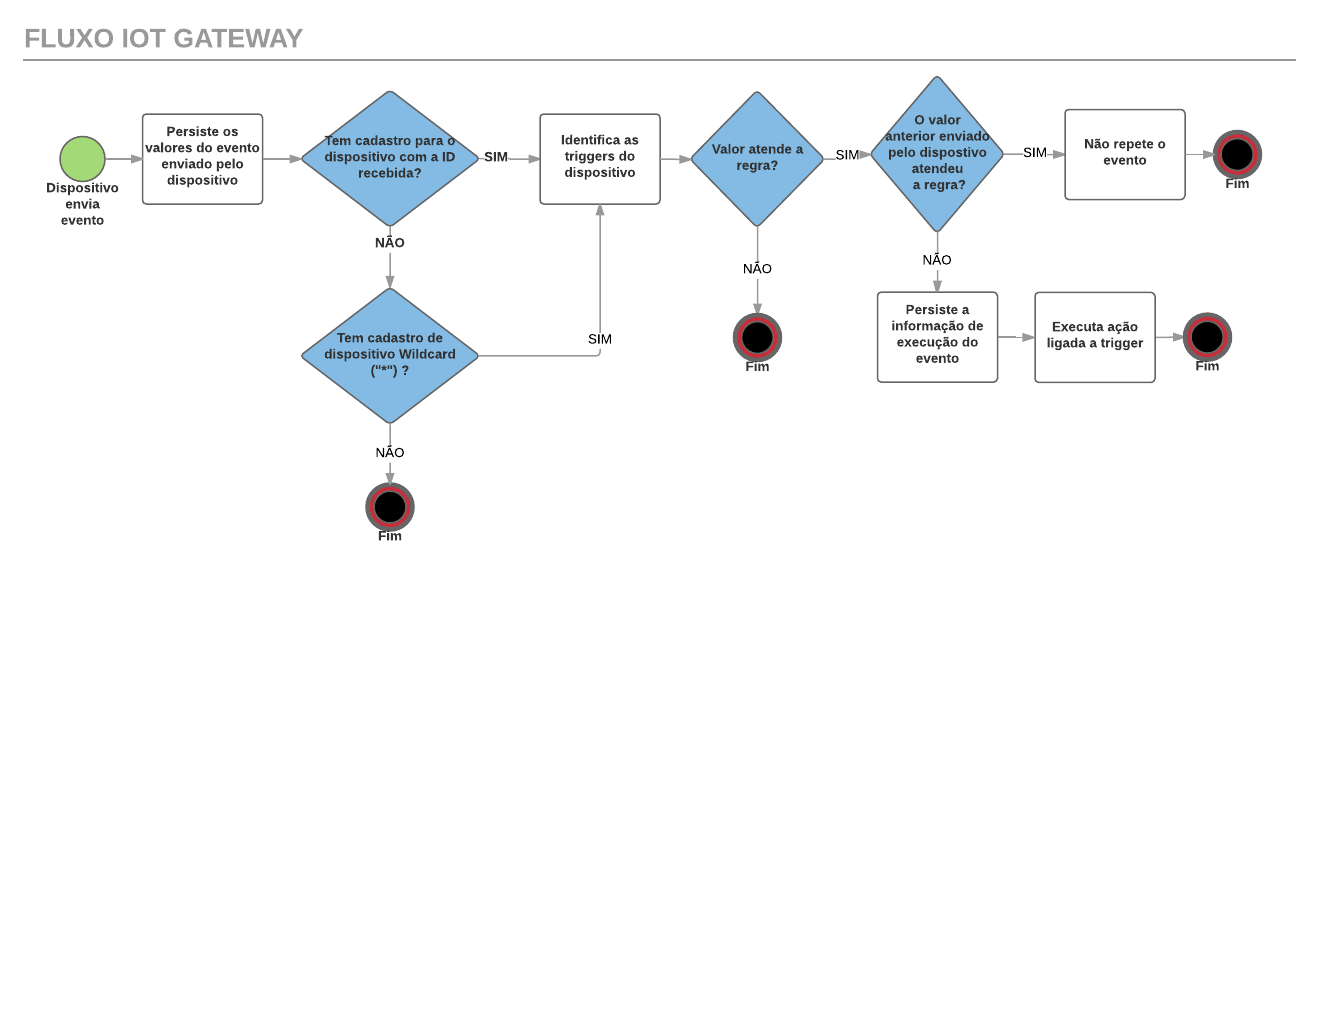
\includegraphics[width=0.9\textwidth]{./img/fluxograma}
		\caption{Representação esquemática do fluxo Gateway IoT.}
		\label{fig:fluxograma}
	\end{center}
\end{figure}

A modelagem desenvolve uma estrutura sequencial que parte da identificação do dispositivo, análise dos gatilhos ligados a este dispositivo, avaliação da operação lógica e liberação para execução do evento, ver Figura~\ref{fig:fluxograma}. Outras entidades não ligadas aos processo principal, visam dar suporte estas operações entregando configurações do sistema e registro de históricos para análise futura. 